\iffalse
\documentclass[journal,12pt,twocolumn]{IEEEtran}

\usepackage[utf8]{inputenc}
\usepackage{kvmap}
\usepackage{graphics} 

\usepackage{setspace}
\usepackage{gensymb}

\singlespacing

\usepackage{amsthm}

\usepackage{mathrsfs}
\usepackage{txfonts}
\usepackage{stfloats}
\usepackage{bm}
\usepackage{cite}
\usepackage{cases}
\usepackage{subfig}

\usepackage{longtable}
\usepackage{multirow}

\usepackage{enumitem}
\usepackage{mathtools}
\usepackage{steinmetz}
\usepackage{tikz}
\usepackage{circuitikz}
\usepackage{verbatim}
\usepackage{tfrupee}
\usepackage[breaklinks=true]{hyperref}
\usepackage{graphicx}
\usepackage{tkz-euclide}
\usepackage{float}

\usetikzlibrary{calc,math}
\usepackage{listings}
    \usepackage{color}                                            %%
    \usepackage{array}                                            %%
    \usepackage{longtable}                                        %%
    \usepackage{calc}                                             %%
    \usepackage{multirow}                                         %%
    \usepackage{hhline}                                           %%
    \usepackage{ifthen}                                           %%
    \usepackage{lscape}     
\usepackage{multicol}
\usepackage{chngcntr}

\DeclareMathOperator*{\Res}{Res}

\renewcommand\thesection{\arabic{section}}
\renewcommand\thesubsection{\thesection.\arabic{subsection}}
\renewcommand\thesubsubsection{\thesubsection.\arabic{subsubsection}}

\renewcommand\thesectiondis{\arabic{section}}
\renewcommand\thesubsectiondis{\thesectiondis.\arabic{subsection}}
\renewcommand\thesubsubsectiondis{\thesubsectiondis.\arabic{subsubsection}}

\hyphenation{op-tical net-works semi-conduc-tor}
\def\inputGnumericTable{}                                 %%

\lstset{
%language=C,
frame=single, 
breaklines=true,
columns=fullflexible
}
\begin{document}

\newtheorem{theorem}{Theorem}[section]
\newtheorem{problem}{Problem}
\newtheorem{proposition}{Proposition}[section]
\newtheorem{lemma}{Lemma}[section]
\newtheorem{corollary}[theorem]{Corollary}
\newtheorem{example}{Example}[section]
\newtheorem{definition}[problem]{Definition}

\newcommand{\BEQA}{\begin{eqnarray}}
\newcommand{\EEQA}{\end{eqnarray}}
\newcommand{\define}{\stackrel{\triangle}{=}}
\newcommand\hlight[1]{\tikz[overlay, remember picture,baseline=-\the\dimexpr\fontdimen22\textfont2\relax]\node[rectangle,fill=blue!50,rounded corners,fill opacity = 0.2,draw,thick,text opacity =1] {$#1$};}
\bibliographystyle{IEEEtran}
\providecommand{\mbf}{\mathbf}
\providecommand{\pr}[1]{\ensuremath{\Pr\left(#1\right)}}
\providecommand{\qfunc}[1]{\ensuremath{Q\left(#1\right)}}
\providecommand{\sbrak}[1]{\ensuremath{{}\left[#1\right]}}
\providecommand{\lsbrak}[1]{\ensuremath{{}\left[#1\right.}}
\providecommand{\rsbrak}[1]{\ensuremath{{}\left.#1\right]}}
\providecommand{\brak}[1]{\ensuremath{\left(#1\right)}}
\providecommand{\lbrak}[1]{\ensuremath{\left(#1\right.}}
\providecommand{\rbrak}[1]{\ensuremath{\left.#1\right)}}
\providecommand{\cbrak}[1]{\ensuremath{\left\{#1\right\}}}
\providecommand{\lcbrak}[1]{\ensuremath{\left\{#1\right.}}
\providecommand{\rcbrak}[1]{\ensuremath{\left.#1\right\}}}
\theoremstyle{remark}
\newtheorem{rem}{Remark}
\newcommand{\sgn}{\mathop{\mathrm{sgn}}}
\providecommand{\abs}[1]{\left\vert#1\right\vert}
\providecommand{\res}[1]{\Res\displaylimits_{#1}} 
\providecommand{\norm}[1]{$\left\lVert#1\right\rVert$}
%\providecommand{\norm}[1]{\lVert#1\rVert}
\providecommand{\mtx}[1]{\mathbf{#1}}
\providecommand{\mean}[1]{E\left[ #1 \right]}
\providecommand{\fourier}{\overset{\mathcal{F}}{ \rightleftharpoons}}
%\providecommand{\hilbert}{\overset{\mathcal{H}}{ \rightleftharpoons}}
\providecommand{\system}{\overset{\mathcal{H}}{ \longleftrightarrow}}
	%\newcommand{\solution}[2]{\textbf{Solution:}{#1}}
\newcommand{\solution}{\noindent \textbf{Solution: }}
\newcommand{\cosec}{\,\text{cosec}\,}
\providecommand{\dec}[2]{\ensuremath{\overset{#1}{\underset{#2}{\gtrless}}}}
\newcommand{\myvec}[1]{\ensuremath{\begin{pmatrix}#1\end{pmatrix}}}
\newcommand{\mydet}[1]{\ensuremath{\begin{vmatrix}#1\end{vmatrix}}}
\numberwithin{equation}{subsection}
\makeatletter
\@addtoreset{figure}{problem}
\makeatother
\let\StandardTheFigure\thefigure
\let\vec\mathbf
\renewcommand{\thefigure}{\theproblem}
\def\putbox#1#2#3{\makebox[0in][l]{\makebox[#1][l]{}\raisebox{\baselineskip}[0in][0in]{\raisebox{#2}[0in][0in]{#3}}}}
     \def\rightbox#1{\makebox[0in][r]{#1}}
     \def\centbox#1{\makebox[0in]{#1}}
     \def\topbox#1{\raisebox{-\baselineskip}[0in][0in]{#1}}
     \def\midbox#1{\raisebox{-0.5\baselineskip}[0in][0in]{#1}}
\vspace{3cm}
\title{\textbf{Optimization Assignment - Advanced} }
\author{Dukkipati Vijay Sai}
\maketitle
\newpage
\bigskip
\renewcommand{\thefigure}{\theenumi}
\renewcommand{\thetable}{\theenumi}
Get Python code for the figure from 
\begin{lstlisting}
https://github.com/dukkipativijay/Fwciith2022/tree/main/Assignment%201/Codes/src
\end{lstlisting}
Get LaTex code from
\begin{lstlisting}
https://github.com/dukkipativijay/Fwciith2022/tree/main/Assignment%201%20-%20Assembly/Codes
\end{lstlisting}
%
\section{Question}
\centering
\textbf{\textit{Q(29),Class 12, CBSE Papers, 2011}}\\
\vspace{0.25cm}
\raggedright
\textbf{
\fi
	There are two types of fertilisers $F_1$ and $F_2$. $F_1$ consists of 10\% Nitrogen and 6\% Phosphoric acidand $F_2$ consists of 5\% Nitrogen and 10\% Phosphoric acid. After testing the soil conditions, a farmer finds that she needs atleast 14 kg of nitrogen and 14 kg of phosphoric acid for her crop. If $F_1$ costs Rs 6/kg and $F_2$ costs Rs 5/kg, determine how much of each type of fertiliser should be used so that nutrient requirements are met at a minimum cost. What is the minimum cost? 
	\\
	\solution
	\begin{figure}[!ht]
		\centering
		\includegraphics[width=\columnwidth]{12/12/2/10/figs/optfig1.png}
		\caption{}
		\label{fig:12/12/2/10}
  	\end{figure}
\iffalse
	}\\
\raggedright
\section{Solution}
\includegraphics[width=0.5\textwidth]{optfig1.png}
\vspace{0.25cm}
\raggedright
Let,\\

\vspace{0.2cm}
x = the number of Kg's of Fertiliser $F_1$\\
\vspace{0.2cm}
y = the number of Kg's of Fertiliser $F_2$\\
\vspace{0.5cm}

\centering
\fi
\begin{table}[!ht]
	\centering
\begin{tabular}{|c|c|c|}
\hline
\textbf{Fertiliser} & \textbf{Nitrogen} & \textbf{Phosphoric Acid} \\
\hline
$F_1$ & 10\% & 6\% \\
\hline
$F_2$ & 5\% & 10\% \\
\hline
Total & 14 kg & 14 kg\\
\hline
\end{tabular}
\caption{}
		\label{table:12/12/2/10}
\end{table}
\iffalse
\vspace{0.25cm}
\raggedright
\\Hence, the problem can be formulated as,\\
\vspace{0.25cm}

\centering

$ 10 \% \hspace{0.1cm}of\hspace{0.1cm} x + 5 \% \hspace{0.1cm}of\hspace{0.1cm}  y \geq 280$\\
\vspace{0.25cm}
$ 6 \%\hspace{0.1cm} of \hspace{0.1cm}x + 10 \% \hspace{0.1cm}of \hspace{0.1cm}y \geq 700$\\
\vspace{0.25cm}
\raggedright
The above equations can be simplified as,\\
\centering
\vspace{0.25cm}
$2x + y \geq 280$\\
\vspace{0.25cm}
$3x + 5y \geq 700$\\
\vspace{0.25cm}
Also, $x \geq 0$, $y \geq 0$\\
\vspace{0.25cm}

\raggedright

Let Z be the total cost of the fertiliser mixture.\\
\vspace{0.25cm}
\centering
$ Z = \min\limits_{x,y} (6x + 5y)$\\
\vspace{0.25cm}
\raggedright
\fi
		The optimization problem can be framed from Table \ref{table:12/12/2/10} as
		\iffalse
The above equations can be expressed in vector form as,\\
\centering
\vspace{0.25cm}
\fi
\begin{align}
	Z = \min_{\vec{x}} \myvec{6&5} \vec{x}\\
\myvec{2&1\\3&5}\vec{x} \preceq \myvec{280\\700}\\
 \vec{x}\succeq  \vec{0} 
\end{align}
yielding
\begin{align}
Z_{min} = Rs. 1000,
\vec{x} = \myvec{100\\80} 
\end{align}

